% 
% Annual CCN conference
% Sample LaTeX Two-Page Summary -- Proceedings Format
% based on the prior cognitive science style file

% Original : Ashwin Ram (ashwin@cc.gatech.edu)       04/01/1994
% Modified : Johanna Moore (jmoore@cs.pitt.edu)      03/17/1995
% Modified : David Noelle (noelle@ucsd.edu)          03/15/1996
% Modified : Pat Langley (langley@cs.stanford.edu)   01/26/1997
% Latex2e corrections by Ramin Charles Nakisa        01/28/1997 
% Modified : Tina Eliassi-Rad (eliassi@cs.wisc.edu)  01/31/1998
% Modified : Trisha Yannuzzi (trisha@ircs.upenn.edu) 12/28/1999 (in process)
% Modified : Mary Ellen Foster (M.E.Foster@ed.ac.uk) 12/11/2000
% Modified : Ken Forbus                              01/23/2004
% Modified : Eli M. Silk (esilk@pitt.edu)            05/24/2005
% Modified : Niels Taatgen (taatgen@cmu.edu)        10/24/2006
% Modified : David Noelle (dnoelle@ucmerced.edu)     11/19/2014
% Modified : Konrad Kording (koerding@gmail.com) 2/15/2017

%% Change "letterpaper" in the following line to "a4paper" if you must. 
% Alternatively, just ignore that because who prints papers anymore?

\documentclass[10pt,letterpaper]{article}

\usepackage{ccn}
\usepackage{pslatex}
\usepackage{apacite}
\usepackage{graphicx}


\title{Context and Causal Structure in Associative Learning}
 
\author{{\large \bf Momchil Tomov, Hayley Dorfman, Samuel Gershman (gershman@fas.harvard.edu)}  \\
  Department of Psychology and Center for Brain Science,\\
  Harvard University, 52 Oxford St., room 295.05\\
Cambridge, MA 02138, USA}


\begin{document}

\maketitle


\begin{quote}
\small
\textbf{Keywords:} 
Bayesian modeling; Associative learning; fMRI; Neuroimaging; Context-dependent learning
\end{quote}

\section{Introduction}

% TODO et al. construct for Kaye1987

Context is ubiquitous, yet its role in learning is poorly understood. Some studies suggest that context is irrelevant in some forms of learning \cite{Kaye1987}. Other studies suggest that context plays the role of an ``occasion setter,'' modulating cue-outcome associations without itself acquiring associative strength \cite{Swartzentruber1995}. Yet other studies suggest that context acts like another punctate cue, entering into summation and cue competition with other cues \cite{Rescorla1984}. \citeA{Gershman2017} reconciled these views within a single model that treats each context role as a distinct causal structure; Bayesian inference can then be used to assign probabilities to each structure based on the training history. The model captured the behavioral pattern of subjects in an associative learning experiment where training history was manipulated to favor particular structures. In this study, we sought to investigate the neural correlates of structure learning in human subjects using fMRI.

\section{Materials and Methods}

\subsubsection{Subjects.}

We recruited 20 healthy subjects (10 female; 19-27 years of age; mean age 22 $\pm$ 2) to participate in this study. Eight additional participants were excluded due to excessive motion or insufficient data.

\begin{figure}[ht]
\begin{center}
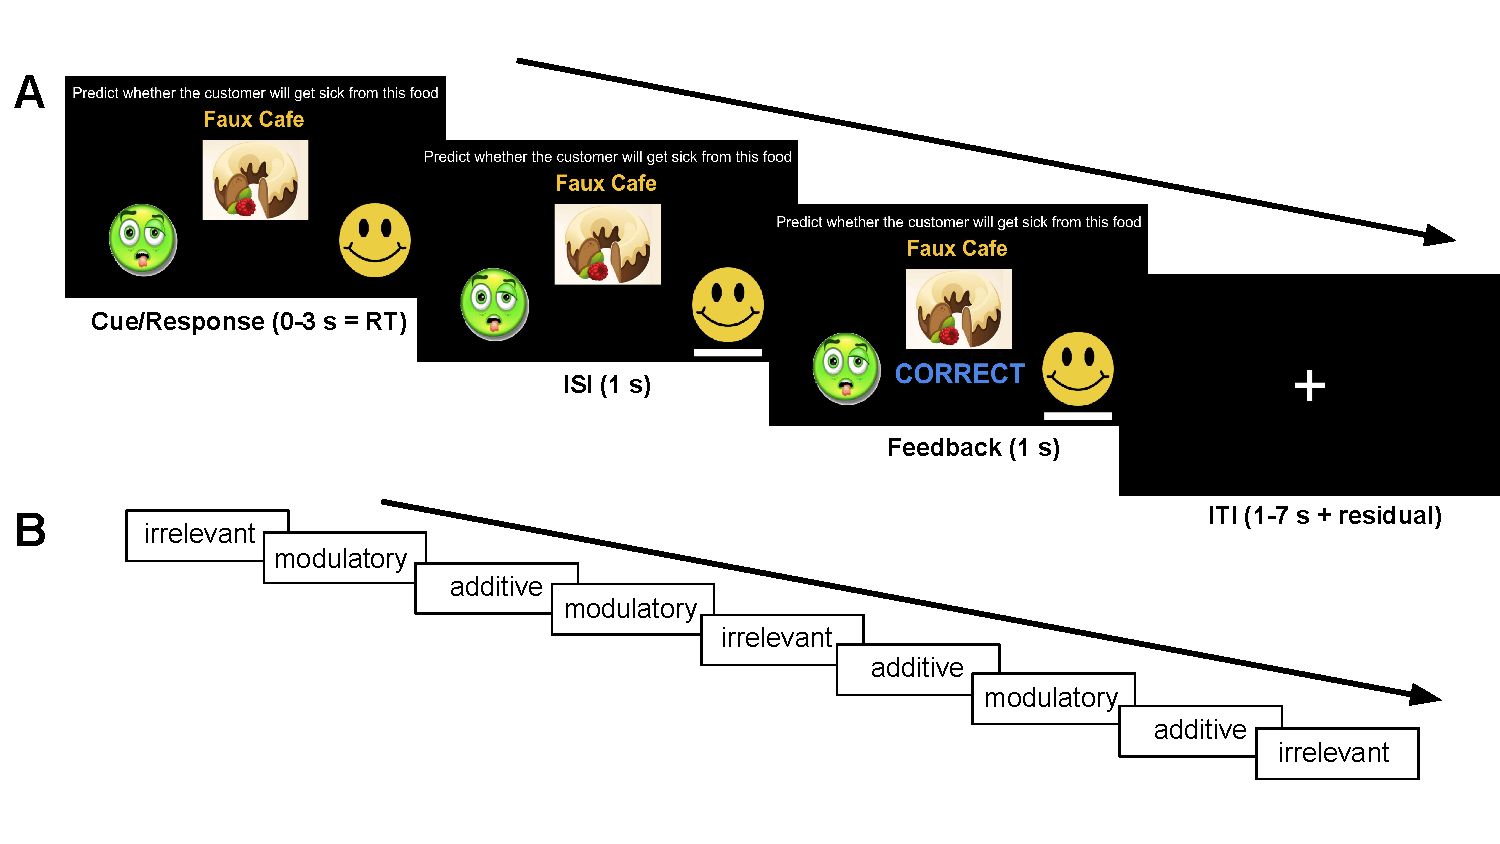
\includegraphics[scale=0.355,  trim = 20 150 0 20]{task-design.pdf}
\end{center}
\vspace{-1em}
\caption{Example timeline of events during a training trial. } 
\label{task-design}
\end{figure}

\subsubsection{Experimental design.} 

We adapted the task used in \citeA{Gershman2017} to a within-subjects design consisting of 9 blocks. Each block consisted of 20 training trials followed by 4 test trials. On each training trial, participants were asked to predict whether a particular food (the cue) in a particular restaurant (the context) would cause sickness (the outcome) and were subsequently informed whether their prediction was correct (Figure~\ref{task-design}). On each test trial, participants were asked to make a prediction about an old or a novel cue in an old or a novel context, without receiving any feedback. The training trials within a block were designed to favor a particular causal structure (irrelevant, modulatory, or additive; Table \ref{table1}). Each condition was presented 3 times in randomized order.
\\

\begin{table}
\centering
\label{table1}
\begin{tabular}{|l|l|l|}
\hline
                     \textbf{Condition}             & \textbf{Training phase}                                                                   & \textbf{Test phase}                                                                   \\ \hline
\textbf{Irrelevant} & \begin{tabular}[c]{@{}l@{}}$x_1c_1+$\\ $x_2c_1-$\\ $x_1c_2+$\\ $x_2c_2-$\end{tabular} & \begin{tabular}[c]{@{}l@{}}$x_1c_1$\\ $x_1c_3$\\ $x_3c_1$\\ $x_3c_3$\end{tabular} \\ \hline
\textbf{Modulatory} & \begin{tabular}[c]{@{}l@{}}$x_1c_1+$\\ $x_2c_1-$\\ $x_1c_2-$\\ $x_2c_2+$\end{tabular} & \begin{tabular}[c]{@{}l@{}}$x_1c_1$\\ $x_1c_3$\\ $x_3c_1$\\ $x_3c_3$\end{tabular} \\ \hline
\textbf{Additive}   & \begin{tabular}[c]{@{}l@{}}$x_1c_1+$\\ $x_2c_1+$\\ $x_1c_2-$\\ $x_2c_2-$\end{tabular} & \begin{tabular}[c]{@{}l@{}}$x_1c_1$\\ $x_1c_3$\\ $x_3c_1$\\ $x_3c_3$\end{tabular} \\ \hline
\end{tabular}
\caption{\textbf{Experimental design}. Cues denoted by ($x_1,x_2,x_3$) and contexts denoted by ($c_1,c_2,c_3$). Outcome presentation denoted by ``$+$'' and no outcome denoted by ``$-$''.}
\end{table}

\subsubsection{Modeling.} 

We implemented the model presented in \citeA{Gershman2017}. The model had two free parameters: the variance $\sigma^2_w$ of the Gaussian prior from which the weights are assumed to be drawn, and the inverse temperature $\beta$ used in the logistic transformation from predictive posterior expectation to choice probability. Intuitively, the former corresponds to the level of uncertainty in the initial estimate of the weights, while the latter reflects choice stochasticity. We fit these parameters using maximum likelihood  estimation based on behavioral data obtained from 10 different subjects who performed the same task outside the scanner during a pilot version of the study. The fitted values were $\sigma^2_w = 0.1249$ and $\beta = 2.0064$. All other parameters had the same values as described in \citeA{Gershman2017}.

\section{Results}

\begin{figure}[ht]
\begin{center}
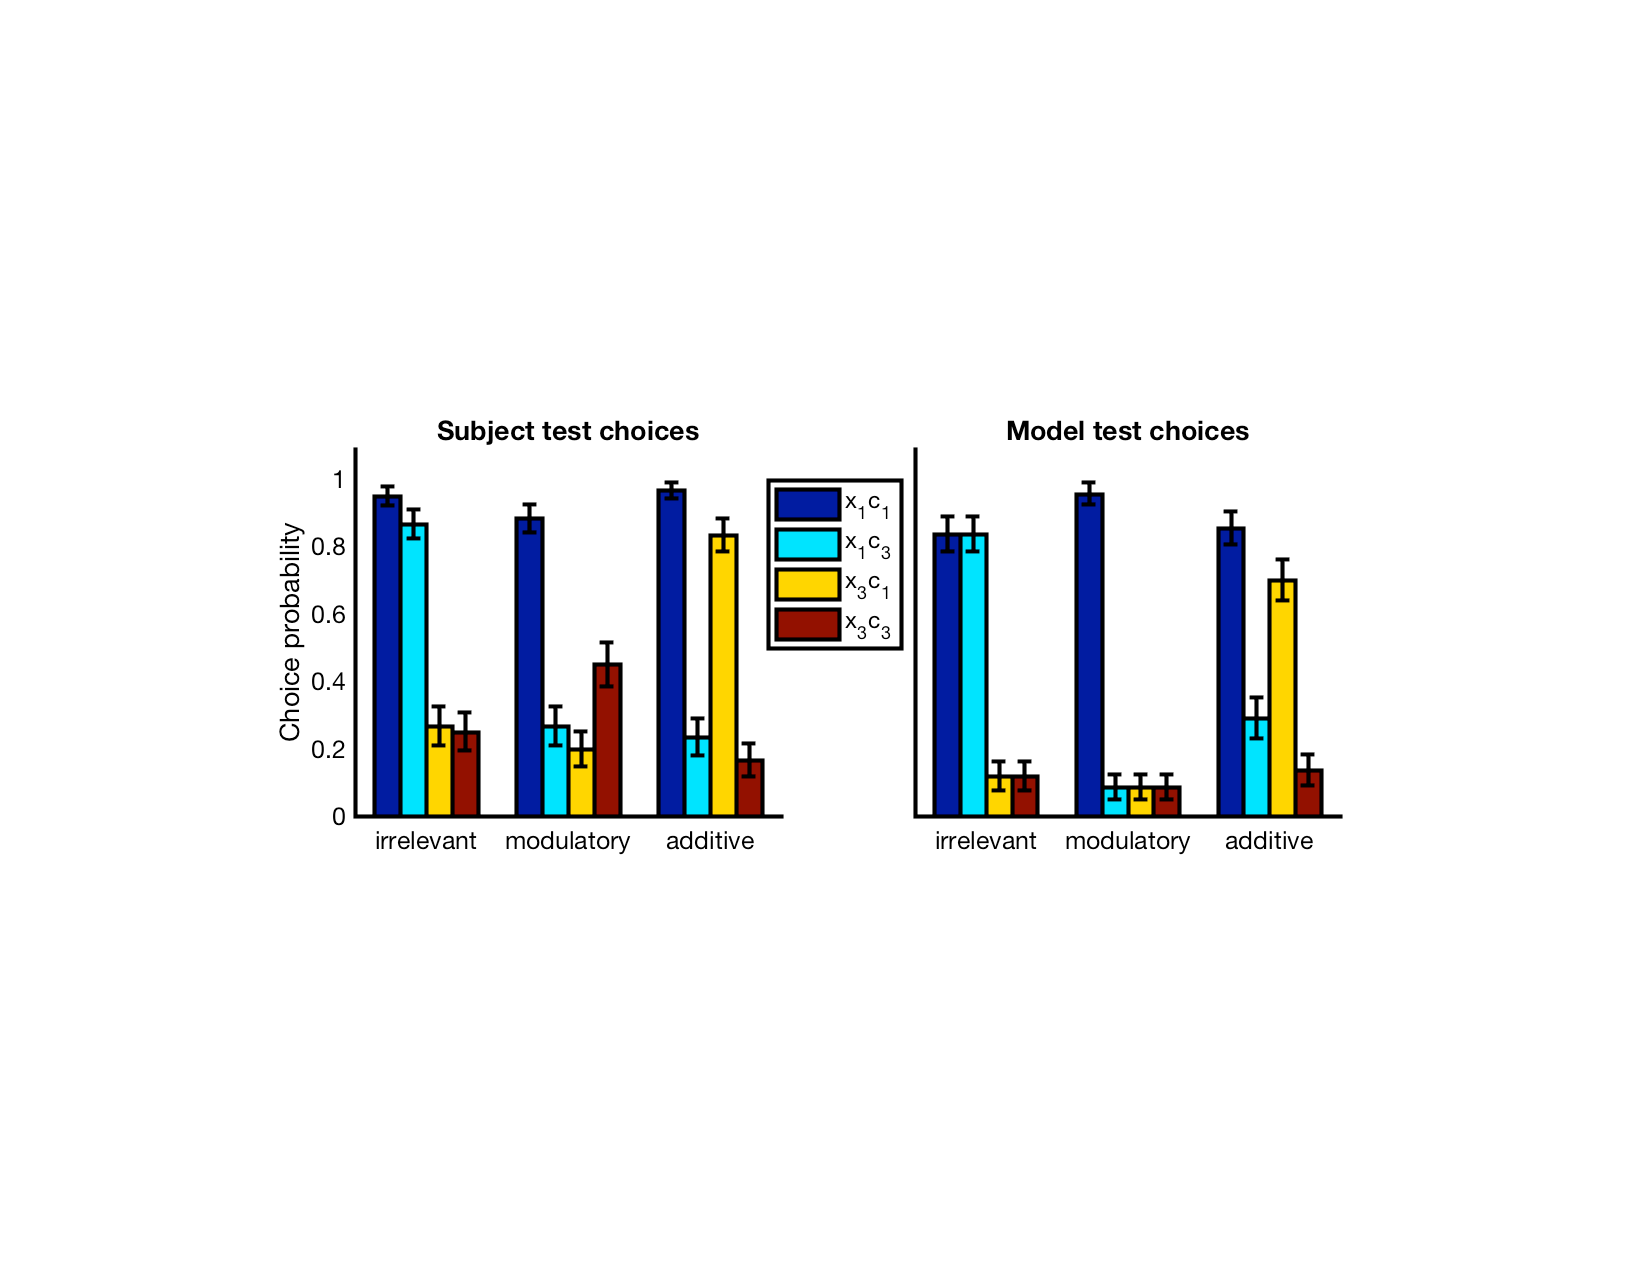
\includegraphics[scale=0.45,  trim = 120 220 120 200]{behavioral.pdf}
\end{center}
\caption{Subject (left) and model (right) performance on the test trials. Each color corresponds to a particular combination of an old ($x_1$) or new ($x_3$) cue in an old ($c_1$) or new ($c_3$) context.} 
\label{behavioral}
\end{figure}

\subsubsection{Behavioral data.}

Participants exhibited the same test trial behavioral patterns (Figure~\ref{behavioral}) in the within-subjects design as previously reported using a between-subjects design \cite{Gershman2017}. The model successfully accounted for participants' choices on both the training and the test trials ($r = 0.7283, p < 0.00001$).

\subsubsection{fMRI data.} 

% SJG: I took out the paragraph and figure below because it's not really clear what to make of this result, at least right now.

% \begin{figure}[ht]
% \begin{center}
% 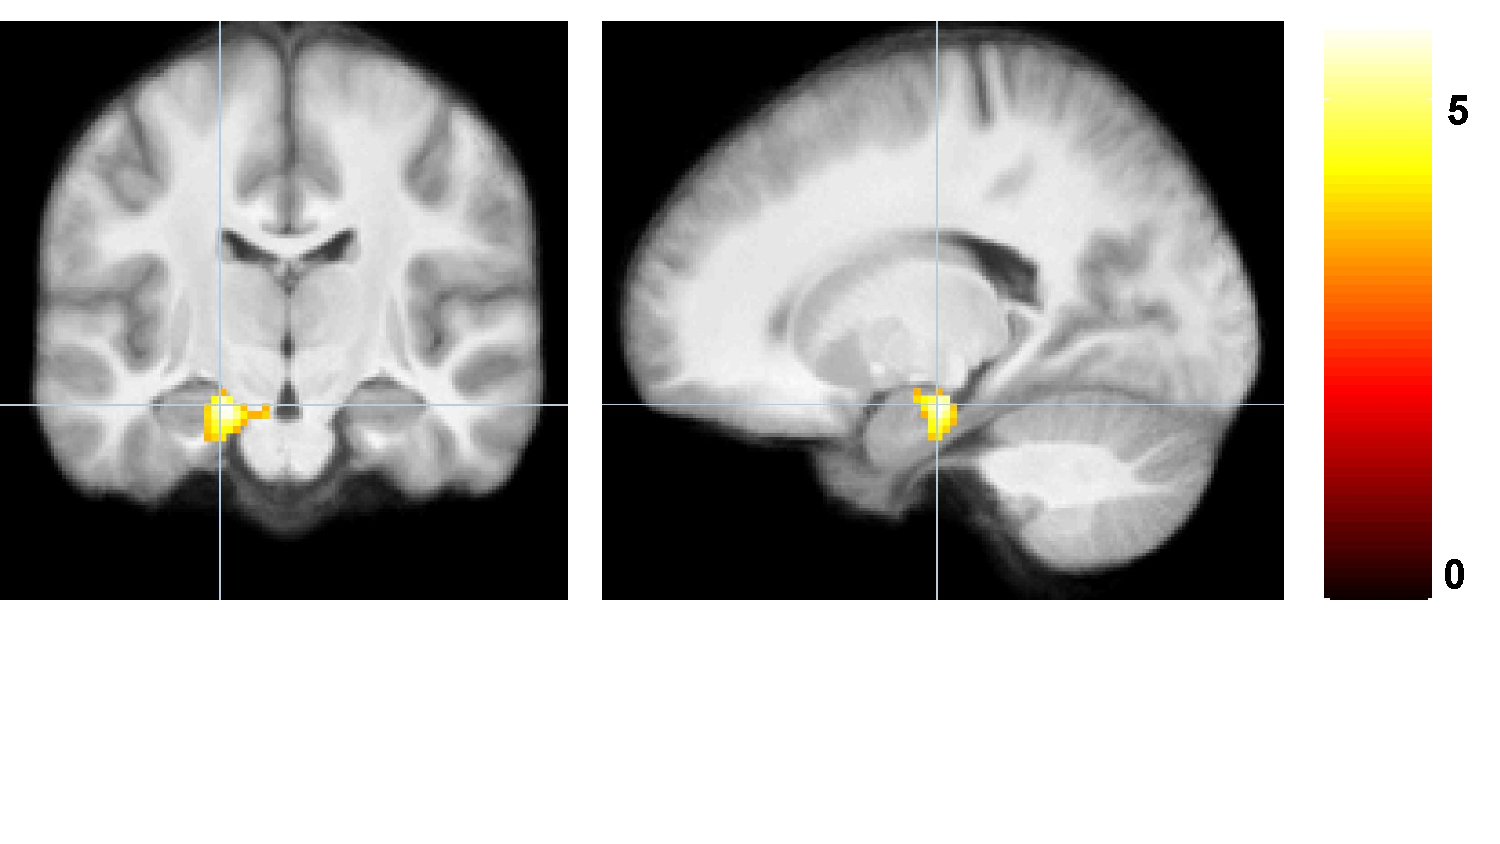
\includegraphics[scale=0.33,  trim = 0 150 0 0]{additive-irrelevant.pdf}
% \end{center}
% \caption{Transient activity related to the additive condition minus the irrelevant condition in left anterior hippocampus (MNI: -18 -16 -18), $t > 3.5518, p < 0.001$, cluster FWE corr. Right: T-value scale.} 
% \label{additive-irrelevant}
% \end{figure}

% We had an a priori hypothesis that the hippocampus would be involved in modulating the cue-outcome association when it is influenced by the context. We therefore contrasted BOLD activation at feedback onset between blocks with different conditions. The BOLD signal did not differ significantly between the modulatory and the irrelevant conditions, nor between the modulatory and the additive conditions. The contrast between the additive and the irrelevant conditions showed increased activation in left anterior hippocampus (Figure~\ref{additive-irrelevant}; MNI coordinates of peak voxel: [-18 -16 -18]; T-value: 5.748; extent with $t > 3.5518$: 141; $p < 0.001$; cluster FWE corrected).

\begin{figure}[ht]
\begin{center}
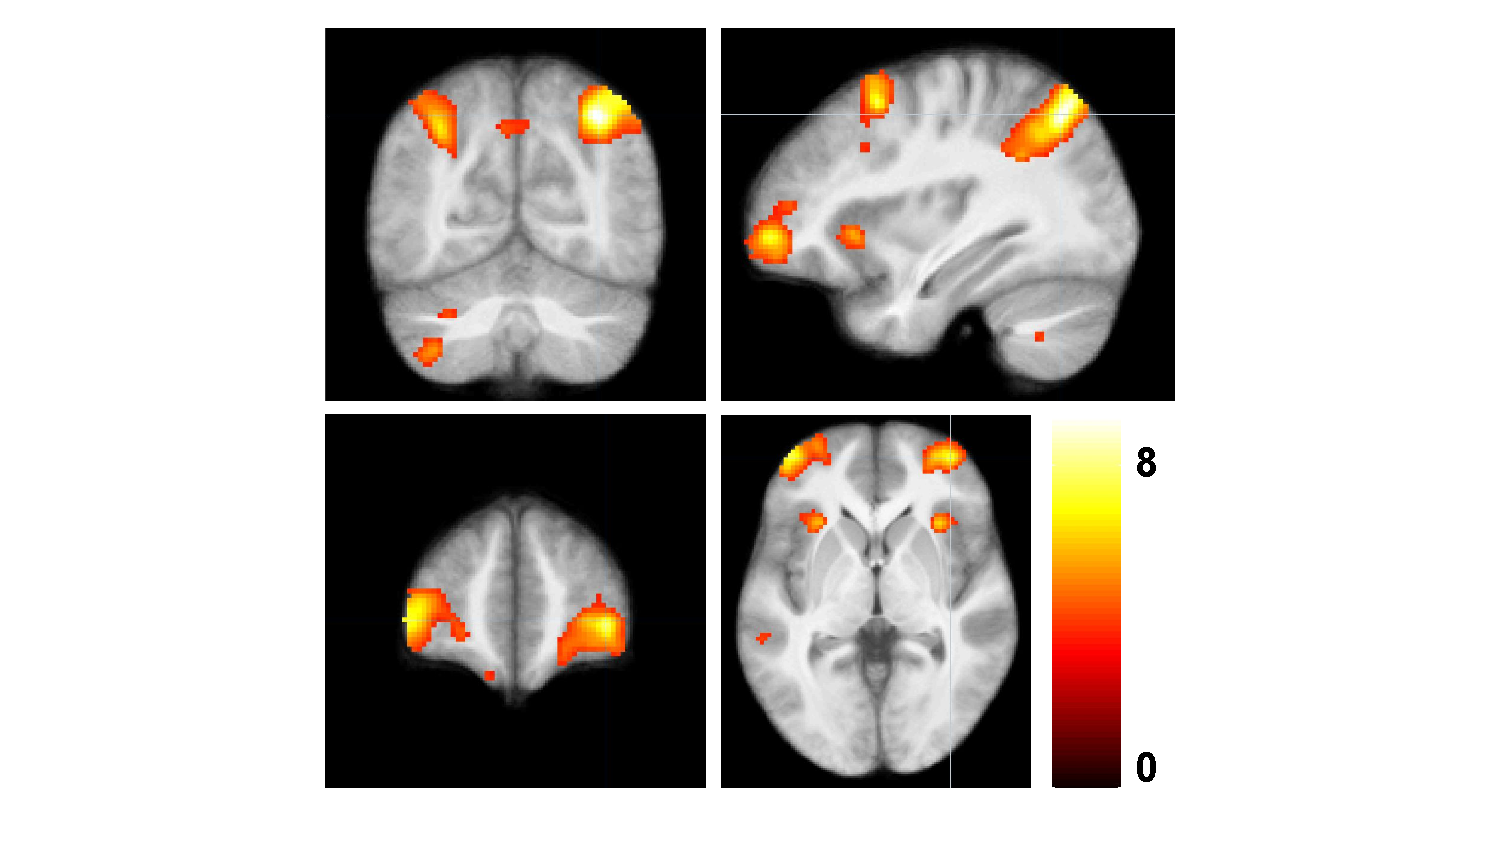
\includegraphics[scale=0.5,  trim = 130 50 0 0]{kl-divergence.pdf}
\end{center}
\caption{Activity tracking the Kullback--Leibler divergence of the posterior over causal structures. Top row: right angular gyrus (MNI: 34 -64 48). Bottom row: right rlPFC (MNI: 48 20 34). $t > 3.5518, p < 0.001$, cluster FWE corr.} 
\label{kl-divergence-img}
\end{figure}

% SJG: I thought there was an mOFC effect here too?

In order to measure the neural correlates of structure learning, we looked for regions that tracked changes in beliefs about the underlying causal structure; specifically, we used the Kullback-Leibler (KL) divergence between the posterior and prior over causal structures as a parametric modulator at feedback onset on each training trial. We found significant bilateral activation in parietal cortex (angular gyri), rostrolateral prefrontal cortex, lateral orbitofrontal cortex, and anterior insula (Figure~\ref{kl-divergence-img}).

% I removed this because it's less essential when you have the brain maps. We'll  use this when we write up a full paper.

% \begin{table}[!ht]
% \begin{center} 
% \caption{Brain activation tracking the KL divergence between the posterior and prior over causal structures. All P-values are $< 0.001$ with cluster FWE correction.} 
% \label{kl-divergence-table} 
% \vskip 0.12in
% \begin{tabular}{llll} 
% \hline
% Brain region    &  Extent & T-value  & MNI coord. \\
% \hline
% Angular gyrus (R) &	484	& 8.638 &	34	-64	48\\
% Inferior frontal gyrus,\\opercular part (R) &	341 &	8.378& 48	 20	34 \\
% Middle frontal gyrus (R) &	130	& 7.440 &	36	56	-2 \\
% Middle frontal gyrus (L) &	173	& 7.205 &	-42	56	2 \\
% Middle frontal gyrus (R) &	86	& 6.996 &	34	12	54 \\
% Inferior parietal gyrus (L) &	254 	& 6.699 &	-30	-54	42 \\
% Superior parietal gyrus (L)	 & 254	& 5.566 &	-34	-72	54 \\
% Inferior frontal gyrus,\\triangular part (L) &	173	& 6.583 & -44	20	22 \\
% Inferior temporal gyrus (R) &	 15	& 6.461 &	60	-24	-20 \\
% Insula (L)	& 18	 & 6.272	& -28	22	-2 \\
% Anterior orbital gyrus (R)& 	8  &	5.827 &	20	48	-16 \\
% \hline
% \end{tabular} 
% \end{center} 
% \end{table}

% SJG: was this cross-validated, or was it literally tested on the last block?

% SJG: you say that performance was at chance; do you mean above chance?

To identify regions containing information about causal structure, we trained a multinomial logistic regression classifier to predict the block condition based on neural activity from a given region at trial onset. We trained the model on the first 8 blocks and evaluated performance on the last block across all subjects. While performance was at chance level for all regions, the hippocampus showed a significant bias towards predicting the modulatory condition ($p < 0.0001$), whereas no significant bias was observed for other regions of interest (orbitofrontal cortex, striatum, and ventromedial prefrontal cortex; $p$'s $> 0.01$). To further investigate this trend, we computed a subject-averaged representation dissimilarity matrix (RDM) using correlation distance of activation patterns from different regions at trial onset. Hippocampal representations of the modulatory condition were more dissimilar from those in the other two conditions ($p < 10^{-6}$, one-way ANOVA and post-hoc t-tests), suggesting that the hippocampus can preferentially distinguish the modulatory causal structure from other structures. The same analysis showed that striatum encoded more distinct representations when the context was irrelevant ($p < 10^{-8}$).

% SJG: Add plots of the classifier and RSA analyses.

\section{Conclusion}

% SJG: add citations

These data suggest that several regions encode information about causal structure, reflecting the role that context plays during learning. Some regions exhibit an inductive bias towards particular structures: hippocampus preferentially signals modulatory conditions, whereas striatum preferentially signals irrelevant conditions. Our results are consistent with previous findings that implicate the hippocampus and the angular gyri in modulating context-dependent associations, with the striatum thought to support a separate stimulus-response learning system.



\bibliographystyle{apacite}

\setlength{\bibleftmargin}{.125in}
\setlength{\bibindent}{-\bibleftmargin}

\bibliography{context_paper.bib}


\end{document}
